\chapter{Konzept}
\label{Konzept}
TODO - Konzept komplett überarbeiten. Siehe 1. Absatz Analyse z.B.

Um die in den Grundlagen beschriebenen Sicherheitsstandards, Protokolle und Integrationslösungen auf ihre Standhaftigkeit in Bezug auf die IT-Schutzziele zu analysieren, werden die Protokolle und Systeme in ihrem Aufbau untersucht und mögliche Schwachstellen herausgearbeitet, daraus hervorgehende Risiken beschrieben und erforderliche Maßnahmen empfohlen. Die \ac{RAMI4.0} beschreibt ein Referenzmodell für Industrie 4.0 Umgebungen. Bereits etablierte Lösungen bestehen aus heterogenen, individuellen Netzwerklandschaften. Um eine Untersuchung der vorhandenen Systeme im neuen Umfeld durchzuführen, müssen verschiedene Faktoren, wie Infrastruktur oder besondere Anforderungen an die Systeme mit einbezogen werden. Das folgende Kapitel dient der Beschreibung der Vorgehensweise bei der Analyse der Netzwerkkommunikation und deren Komponenten.

\section{Komponenten}
Die beschriebenen Anforderungen müssen, um eine sichere Netzwerkkommunikation zu gewährleisten, von allen beteiligen Komponenten der Umgebung integriert und umgesetzt werden. Industrie 4.0 Umgebungen können in unterschiedlichster Form ausgeprägt sein. Die Umsetzung der Hard- und Softwarekomponenten hängt von den zu übertragenden Daten, dem Übertragungsmedium, der Übertragungsdistanz und vorausgesetzten Dienstgüte ab. Die zu analysierenden Komponenten werden in Hard- und Softwarekomponenten gegliedert.

\subsection{Hardware}

TODO

\subsubsection{Übertragungskanal}
Der Übertragungskanal beschreibt die Bitübertragungsschicht. In Industrie 4.0 Umgebungen ist es notwendig, Daten zu übertragen, um eine räumliche oder zeitliche Distanz zu überbrücken. Je nach Anwendungsfall findet diese Kommunikation über Kupfer- bzw. Glasfaserkabel, Funkübertragung oder ein Speichermedium statt. Je nach Beschaffenheit des Übertragungskanals, ist es notwendig, weitere Maßnahmen zur Sicherheit der Kommunikation zu treffen. Aufgrund der Durchführung der Analyse in einem virtuellen Testsystem, werden die Auswirkungen der Form des Übertragungskanals bei der Analyse der Kommunikation nicht beachtet.

\subsection{Software}
Jede Komponente einer \ac{ICS}-Umgebung kann Softwareschwachstellen und Sicherheitslücken enthalten. Dabei spielt es keine Rolle, ob es sich um ein komplexes \ac{ICS} handelt oder um einen einfachen Anwendungsserver. Software-Aktualisierungen sowie ein Patch-Management sind für einen sicheren Betrieb notwendig, um Angriffe über Exploits zu verhindern. 

\subsubsection{Netzwerkstack}
Die Kommunikation zwischen Industrieanlagen findet mehr und mehr auf der Basis von TCP-basierten Netzwerken statt. Das \ac{RAMI4.0} beschreibt Industrie 4.0 Umgebungen als \ac{SOA}. \ac{SOA} beschreibt ein Netzwerk, in welchem von den Teilnehmern Dienste bereitgestellt und genutzt werden können. Die Dienste im Netzwerk werden i. d. R. über eine \ac{REST}-\ac{API} bereitgestellt. Diese Schnittstellen nutzen bereits etablierte Protokolle der \ac{IoT} oder \ac{IIoT} Welt.

\subsubsection{Protokolle}
\ac{IoT}-Geräte nutzen das Internet als Übertragungsmedium. Somit müssen sie zur Übertragung ihrer Daten Protokolle nutzen, welche die Internet Protocol Suite der \ac{IETF} einhalten. Etablierte Internet-Protokolle wie HTTP und XMPP wurden zur Kommunikation ressourcenreicher Geräte mit hoher Leistung entwickelt und sind für viele Netzwerke mit \ac{IoT}- oder \ac{IIoT}-Endknoten zu komplex, bzw. nicht geeignet. Im Rahmen der 4. industriellen Revolution wurden daher, vor allem für \ac{IIoT} Umgebungen, neue Protokolle entwickelt, welche ressourcensparende, sichere Kommunikation zwischen Maschinen bereitstellen sollen. 

TODO - CoAP, MQTT

\section{Abgrenzung}
\label{Konzept:Abgrenzung}
Die \ac{IIRA} ist ein anerkannter, in der Industrie verbreiteter Standard. Da die Analyse der Netzwerksicherheit am in \autoref{Grundlagen:Testsystem} beschriebenen Testsystem durchgeführt werden soll, welches den Kommunikationsstandard \ac{OPC UA} implementiert, wird sich im weiteren Verlauf der Thesis ausschließlich auf die in der IEC 62541 beschriebene Architektur \ac{RAMI4.0} als Referenzmodell zur Analyse bezogen. Es werden Bedrohungen in Industrie 4.0 Umgebungen beschrieben, eine Analyse der Übertragungsmedien und Infrastruktur durchgeführt und die im Testsystem verwendeten Protokolle mit Bezug auf ihre Anforderungen im Bereich der Netzwerksicherheit untersucht. Um verschiedene Praxisszenarien darzustellen, wird das Testsystem um für die Analyse benötigte, zusätzliche Komponenten erweitert. 

\section{Anpassungen}
\label{Konzept:Anpassungen}
TODO GEHT NIX DOCKER

\section{Vorgehensweise}
Die Analyse der Netzwerkkommunikation der unteren Schichten (Internet- und Link Layer) des im \autoref{Grundlagen:TCP/IP Referenzmodell} beschriebenen TCP/IP Referenzmodells wird auf Basis der in \autoref{Grundlagen:Grundprinzipien der sicheren Kommunikation} erläuterten Schutzziele durchgeführt. Die oberen Schichten (Transport- und Application Layer) werden in der Testumgebung durch das \ac{M2M}-Protokoll \ac{OPC UA} realisiert. Hierbei dient die Spezifikation des Protokolls als Grundlage der Analyse. Aus der Spezifikation ergeben sich die bei der Kommunikation für die IT-Sicherheit zuständigen Komponenten von \ac{OPC UA}. Diese werden nach des Anforderungen des TODO - ref. BSI ICS Security Kompendium und FIRST CVSS v2.0 - auf Sicherheitslücken und Widersprüche untersucht. Bei der Analyse auftretende, mögliche Schwachstellen werden in einer vorhandenen, prototypischen Industrie 4.0 Testumgebung \cite{Weber2018} implementiert und nachgewiesen. Sicherheitslücken, welche durch Fehlkonfiguration auftreten und keine konzeptionellen Schwachstellen der Software oder deren Protokolle darstellen, sollen in der Testumgebung aktiviert und deaktiviert werden können, um die Auswirkung eines Angriffs auf ein Industrie 4.0 System zu Lehr- und Testzwecken darstellen zu können.

\section{Fehlgeschlagene Konzepte/Konzeptwahl}

\begin{figure}[h]
    \centering
    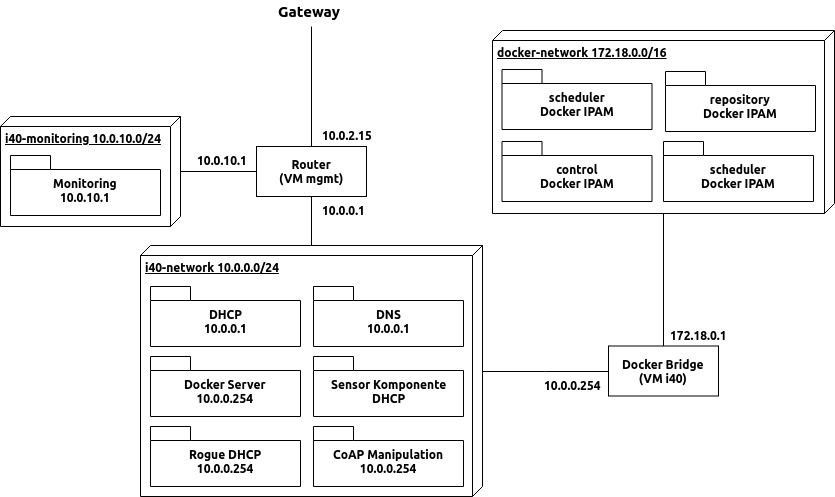
\includegraphics[width=15cm]{netzwerk}
    \caption{Netzwerkinfrastruktur} 
    \label{Konzept:Netzwerkkonzept}
  \end{figure}
  
  \clearpage

  \begin{figure}[h]
    \centering
    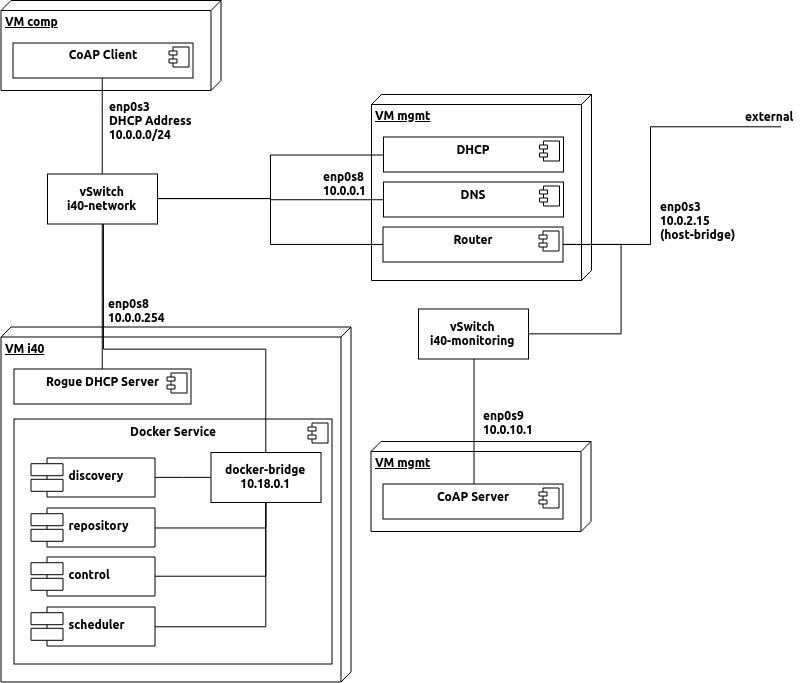
\includegraphics[width=15cm]{vm}
    \caption{Kommunikation der virtuellen Maschinen} 
    \label{Konzept:VMKommunikation}
  \end{figure}
  
  \clearpage